\documentclass[a4paper,11pt]{jsarticle}

%まず使用するパッケージ
\usepackage{amsmath, amsfonts, amssymb, mathtools, mathrsfs, latexsym}
\usepackage{nccmath, empheq}

%\usepackage[draft]{graphicx}
\usepackage[dvipdfmx]{graphicx}
\usepackage[dvipdfmx]{color}
\usepackage{here, wrapfig, subcaption}
\usepackage{enumerate, comment, fancyhdr}
\usepackage{otf}
%mathtoolsを用いたコマンド定義
\DeclarePairedDelimiter{\abs}{\lvert}{\rvert}

\usepackage{seiritz}

\pagestyle{fancy}
  \lhead{2023/12/16}
  \rhead{第2問}
  \cfoot{\thepage}

%%%%%%%%%% メイン %%s%%%%%%%%
\begin{document}
\qSentence{第2問}
%!TEX root = *.tex
%%%%%%%%%%%%%%%%%%
% カウンタのリセット
\setcounter{figure}{0}
% 問題文
図1のように,鉛直上向きで一様な磁束密度$B$の磁場中に,
距離$l$だけ離れた平行な2本の長い導体レールが水平面から角度$\theta\,(0^\circ <\theta <90^\circ)$だけ傾けて固定されている.
導体レールの上端は長さ$l$の細い一様な抵抗線$\text{P}^\prime\text{Q}^\prime$で接続されており,導体レールには,質量$M$,長さ$l$の細い導体棒$\text{PQ}$がそれぞれの導体レールに対して垂直に置かれ,回路を構成している.
この回路に関する以下の問いに答えなさい.
ただし,導体棒と導体レールの間の摩擦や空気抵抗,および抵抗線以外の電気抵抗は無視でき,導体棒は回転しないものとする.
また,回路を流れる電流がつくる磁場は無視できるものとする.
解答においては,抵抗線を$\text{Q}^\prime$から$\text{P}^\prime$へ向かう向きを自由電子(以下,電子と書く)の速度や電流の正の向き,レールに沿って下向きを導体棒の速度の正の向きとしなさい.
また,重力加速度の大きさを$g$とする.電子の電荷を$-e$(ただし,$e>0$),質量を$m$とする.

ある時刻に導体棒は,レールに沿って下向きに速さ$v$で運動していた.


\begin{enumerate}[(1)]
  \setlength{\leftskip}{-1zw}
  \setlength{\itemindent}{1zw}\setlength{\labelsep}{0.5zw}
  \setlength{\labelwidth}{1zw}\setlength{\leftmargin}{1zw}
  \setlength{\itemsep}{0.5\baselineskip}
  \item この導体棒の運動によって発生する誘導起電力を求めなさい.
  \item 誘導起電力によって,抵抗線中に一様な電場が発生した.この電場の大きさを求めなさい.
\end{enumerate}

抵抗線中の電子の運動から抵抗線の抵抗値について考える.
電子の速度を$c$としたとき,電子は速度に比例する抵抗力$-kc$を受けるものとする.
抵抗線中の単位長さあたりの電子の個数を$n$とする.

\begin{enumerate}[(1)]
  \setlength{\leftskip}{-1zw}
  \setlength{\itemindent}{1zw}\setlength{\labelsep}{0.5zw}
  \setlength{\labelwidth}{1zw}\setlength{\leftmargin}{1zw}
  \setlength{\itemsep}{0.5\baselineskip}
  \addtocounter{enumi}{2}
  \item 抵抗線に沿って運動する電子の加速度を$a$として,電子1個に対する運動方程式を$e,\,v,\,B,\,\theta,\,m,\,a,\,k,\,c$を用いて表しなさい.
\end{enumerate}

電子の速度$c$は,十分時間が経った後に速度$c_1$のまま時間変化しなくなった.

\begin{enumerate}[(1)]
  \setlength{\leftskip}{-1zw}
  \setlength{\itemindent}{1zw}\setlength{\labelsep}{0.5zw}
  \setlength{\labelwidth}{1zw}\setlength{\leftmargin}{1zw}
  \setlength{\itemsep}{0.5\baselineskip}
  \addtocounter{enumi}{3}
  \item このときの電子の速度$c_1$を$e,\,v,\,B,\,\theta,\,k$を用いて表しなさい.
  \item 抵抗線中の電子の集団が速度$c_1$で運動することによる電流$I$を$e,\,m,\,k,\,c_1,\,n$のうち必要な記号を用いて表しなさい.
  \item 抵抗線$\text{P}^\prime\text{Q}^\prime$の抵抗値を$e,\,k,\,n,\,l$を用いて表しなさい.
  \item 抵抗線中で電子の速度に比例する抵抗力が単位時間あたりに電子1個に対してする仕事$W$,および単位時間あたりに発生する熱量$J$を,それぞれ$e,\,v,\,B,\,\theta,\,k,\,n,\,l$のうち必要な記号を用いて表しなさい.
\end{enumerate}

次に,図2のように抵抗線を自己インダクタンス$L$のコイルに取り替えた.
時刻$t=0$における導体棒の位置を原点とし,レールに沿って下向きに\x 軸を取った.
時刻$t=0$において静止していた導体棒を静かにはなした後の運動について考える.
導体棒が位置\x にあるとき短い時間$\Delta t$の間の位置の変化を$\Delta x$とし,このときの電流の変化を$\Delta I$とする.
なお,$t=0$において電流は流れていなかった.
また,コイル以外の自己インダクタンスは無視できるものとする.

\begin{enumerate}[(1)]
  \setlength{\leftskip}{-1zw}
  \setlength{\itemindent}{1zw}\setlength{\labelsep}{0.5zw}
  \setlength{\labelwidth}{1zw}\setlength{\leftmargin}{1zw}
  \setlength{\itemsep}{0.5\baselineskip}
  \addtocounter{enumi}{7}
  \item 電流と導体棒の位置の変化は$\Delta I=D\Delta x$と表すことができる.$D$を$B,\,\theta,\,l,\,L$を用いて表しなさい.
\end{enumerate}

前問により,任意の時刻の電流は$I=Dx$と表せることがわかる.

\begin{enumerate}[(1)]
  \setlength{\leftskip}{-1zw}
  \setlength{\itemindent}{1zw}\setlength{\labelsep}{0.5zw}
  \setlength{\labelwidth}{1zw}\setlength{\leftmargin}{1zw}
  \setlength{\itemsep}{0.5\baselineskip}
  \addtocounter{enumi}{8}
  \item 導体棒が位置\x にあるときの導体棒の加速度を$A$として\x 軸方向についての運動方程式を$M,\,A,\,g,\,B,\,\theta,\,l,\,L,\,x$を用いて表しなさい.
  \item 導体棒は単振動をし,導体棒の位置は$x=\alpha +\beta\cos{\omega t}$\,(ただし,$\omega>0$)と表すことができる.$\alpha,\,\beta,\,\omega$をそれぞれ$M,\,g,\,B,\,\theta,\,l,\,L$のうち必要な記号を用いて表しなさい.
  \item 前問のように導体棒の位置が表されるとき,その速度は$-\omega\beta\sin\omega t$と表すことができる.時刻$t$において,コイルに蓄えられているエネルギーと導体棒の力学的エネルギーの合計を求めなさい.ただし,導体棒の位置エネルギーの基準点は$x=0$とする.また,\underline{解答には$M,\,L,\,\alpha,\,\beta,\,\omega$を用いないこと}.
\end{enumerate}

\begin{figure}[H]
  \centering
  \begin{minipage}{.3\columnwidth}
    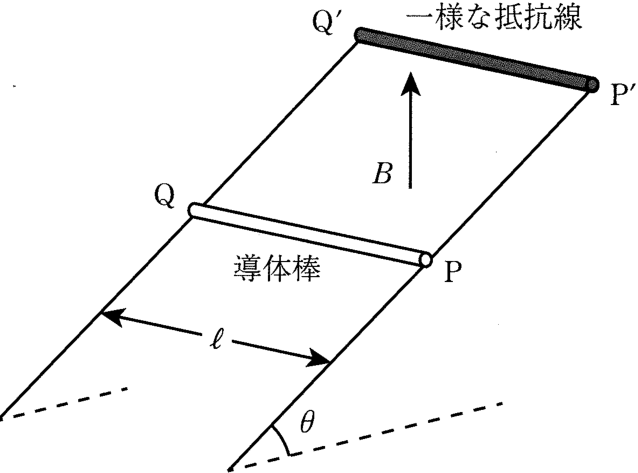
\includegraphics[width=\columnwidth]{../graphs/chiba_23_4-1.png}
    \caption{}
  \end{minipage}
  \hspace{.1\columnwidth}
  \begin{minipage}{.3\columnwidth}
    \centering
    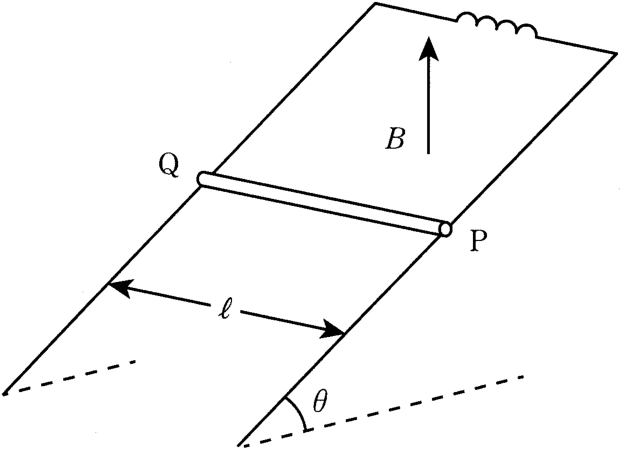
\includegraphics[width=\columnwidth]{../graphs/chiba_23_4-2.png}
    \caption{} 
  \end{minipage}
\end{figure}






% メモ
\begin{comment}

\end{comment}


%%%%%%%%%%%%%%%%%%

\hruleline
%\input{../prac_exam/open_19_8/Q2_sol.tex}
\end{document}